\subsection{Dose–response analyses during the session}

\paragraph{Global dose–response by molecule.}
Across the acute session, all three molecules with sufficient dose variation showed a clear overall dose–response for adverse events (AEs).
Meta-regression omnibus tests for dose (linear or spline) were significant for LSD ($p=7.49\times10^{-4}$), MDMA ($p=2.31\times10^{-2}$), and psilocybin ($p=1.22\times10^{-5}$), indicating that higher doses were associated with higher AE burden at the session level (Table~\ref{tab:dr-global-by-molecule}).
Visual inspection of the global curves (Fig.~\ref{fig:dr-global-session}) shows a steeper overall rise for psilocybin, a robust increase for MDMA that is close to linear over the studied range, and a non-linear shape for LSD consistent with a marked increase at the upper end of its tested doses.

\begin{figure}[htb]
  \centering
  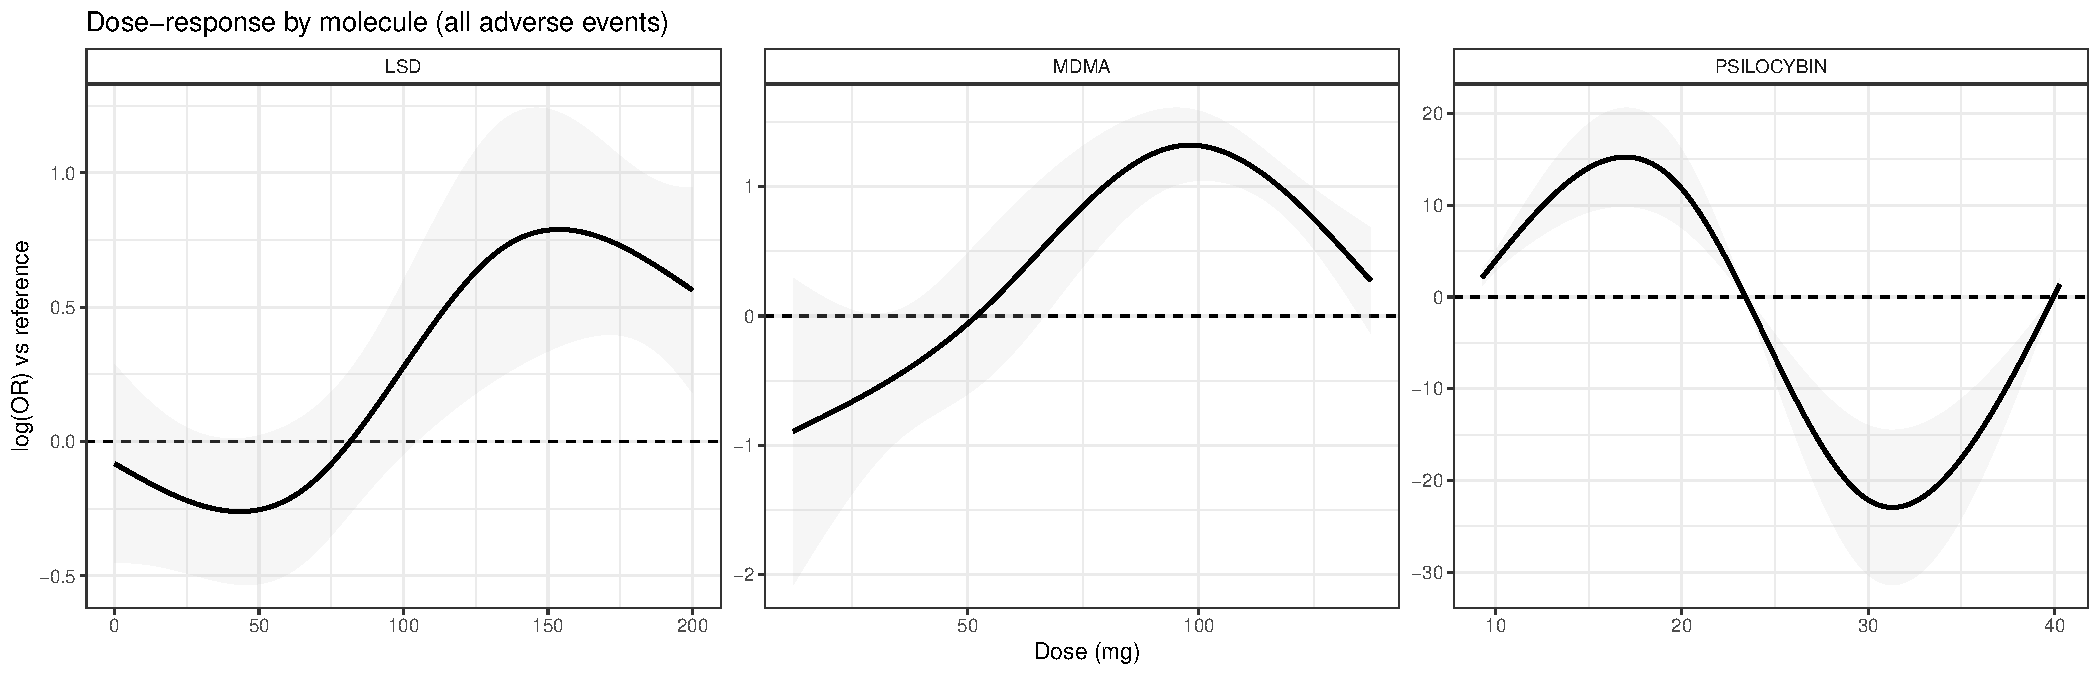
\includegraphics[width=0.94\textwidth]{figures/master_dr_by_molecule-session.pdf}
  \caption{\textbf{Global dose–response during session by molecule.}
  Modeled log-odds ratio (log(OR)) of experiencing any AE across dose for LSD, MDMA and psilocybin during the acute session. Shaded bands are 95\% CIs.}
  \label{fig:dr-global-session}
\end{figure}

\begin{table}[htbp]
  \centering
  \caption{Global session dose--response tests by molecule.}
  \label{tab:dr-global-by-molecule}
  \begin{tabular}{lcccc}
    \toprule
    Molecule & $k_{\text{session}}$ & $Q_M$ & $p$ & Sig. \\
    \midrule
    LSD & 149 & 11.36 & 7.49e-04 & *** \\
    MDMA & 197 & 5.16 & 2.31e-02 & * \\
    PSILOCYBIN & 162 & 19.13 & 1.22e-05 & *** \\
    \bottomrule
  \end{tabular}
\end{table}


\paragraph{Dose–response by specific adverse event (AE).}
Session-specific meta-regressions isolated the AE terms with statistically reliable dose gradients (Table~\ref{tab:dr-ae-by-molecule-session}).
Figure~\ref{fig:dr-by-ae-session} visualizes the corresponding slopes.
Only a handful of terms crossed the $p<0.05$ threshold once multiplicity was controlled, underscoring that most AEs behave as threshold phenomena rather than dose-proportional hazards.

For \textbf{LSD}, significant dose effects were confined to \textit{nausea} ($p=3.17\times10^{-3}$), \textit{headache} ($p=1.18\times10^{-2}$), and \textit{visual illusions} ($p=4.94\times10^{-2}$).
All three slopes were positive, indicating that incremental milligram increases within the 50--200\,\textmu g range steadily heightened somatic discomfort and perceptual distortion.
No cognitive or affective AEs met the significance threshold, implying that LSD’s mental-state shifts may be more binary once psychedelic doses are reached, whereas gastrointestinal strain scales with exposure.

For \textbf{MDMA}, two physiologic AEs retained significant slopes: \textit{headache} ($p=3.83\times10^{-2}$) and \textit{dizziness} ($p=4.87\times10^{-2}$).
Both effects rose linearly across the 50--125\,mg span and mirror the sympathetic activation profile reported in controlled MDMA sessions.
Other autonomic terms (e.g., jaw tension, perspiration) trended upward but did not meet the corrected threshold, suggesting either greater between-study heterogeneity or limited power for those endpoints.

For \textbf{psilocybin}, a restricted cubic spline captured a pronounced non-linear relation for \textit{fatigue} ($p=2.54\times10^{-6}$), with risk inflecting sharply at doses above 25\,mg.
In addition, \textit{hypertension/blood-pressure elevation} showed a significant linear effect ($p=4.07\times10^{-3}$).
These results align with clinical observations that psilocybin’s tolerability hinges on cardiovascular monitoring and energy conservation strategies.

No molecule exhibited significant negative slopes, and ayahuasca did not yield analyzable dose variability; its studies used essentially standardized brew volumes.
Taken together, the AE-level findings demonstrate that only a small subset of adverse events scale meaningfully with dose, and these are predominantly somatic or autonomic in nature.


\begin{figure}[htb]
  \centering
  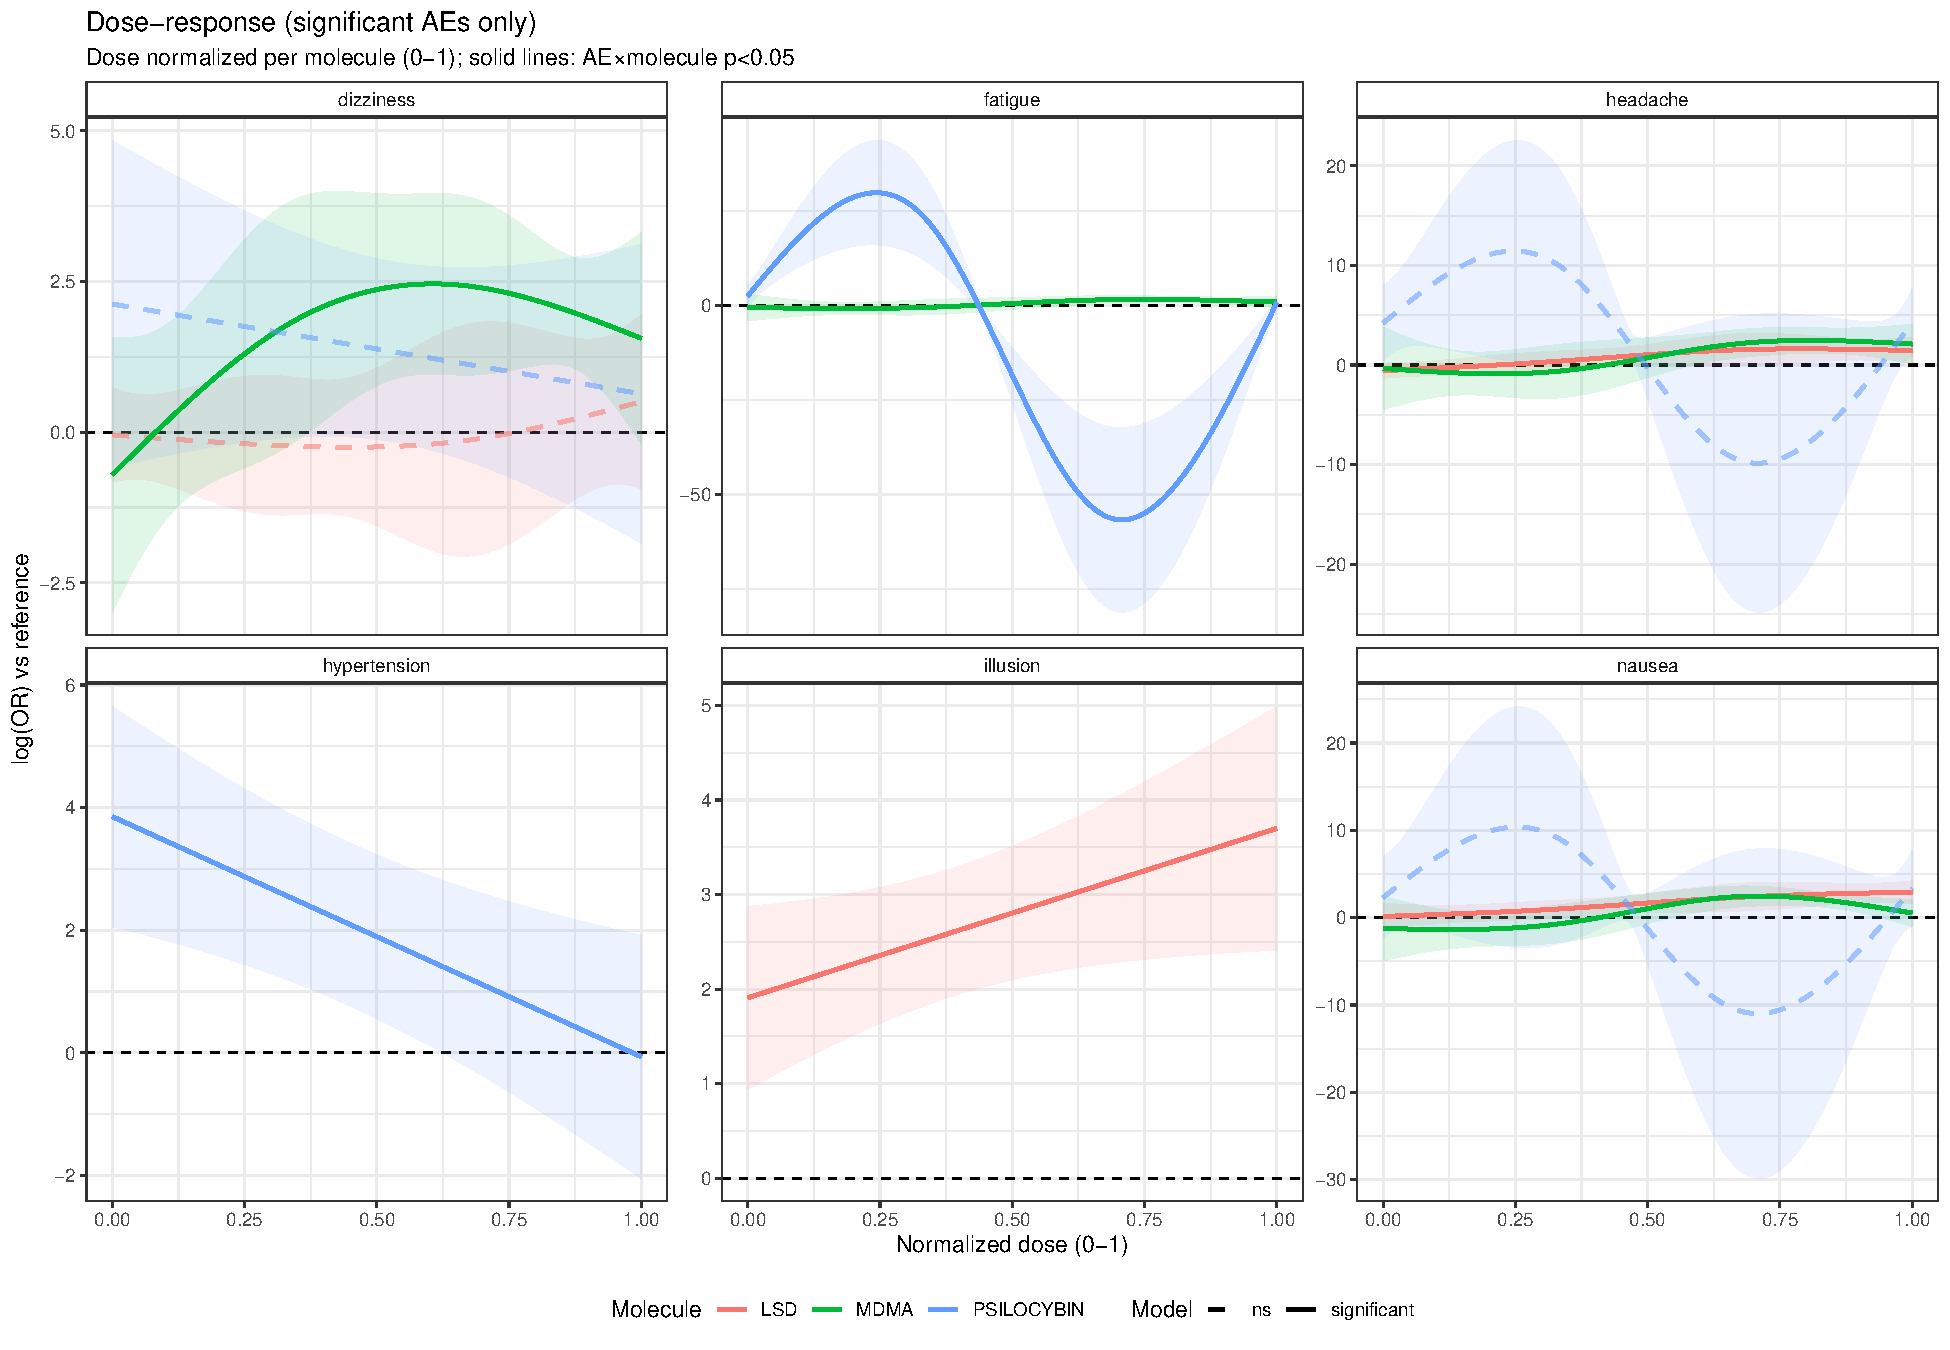
\includegraphics[width=0.94\textwidth]{figures/master_dr_by_ae-session.pdf}
  \caption{\textbf{Per-AE dose–response during session (facets).}
  For each adverse event (facet), modeled log(OR) vs.\ dose is shown by molecule. Stars in the original panels indicate AE$\times$dose significance (p\,$<\,$0.05).}
  \label{fig:dr-by-ae-session}
\end{figure}

\paragraph{Session vs.\ follow-up dose–response (molecules with longitudinal data).}
LSD and MDMA were the only molecules with analyzable follow-up assessments.
Figure~\ref{fig:dr-session-followup} contrasts their global dose–response slopes across windows.
LSD displayed a positive slope during the session ($p=7.49\times10^{-4}$) but a modest \emph{negative} slope at follow-up ($p=3.01\times10^{-2}$), indicating that higher session doses were not associated with lingering AE burdens and may even accelerate resolution of mild sequelae.
MDMA maintained a significant session slope ($p=2.31\times10^{-2}$) yet showed no residual dose effect after the session ($p=0.41$).
These findings clarify that the most robust dose dependencies are confined to the acute dosing day, with no evidence for sustained dose scaling of AEs in the post-session window for either drug.

\begin{figure}[htb]
  \centering
  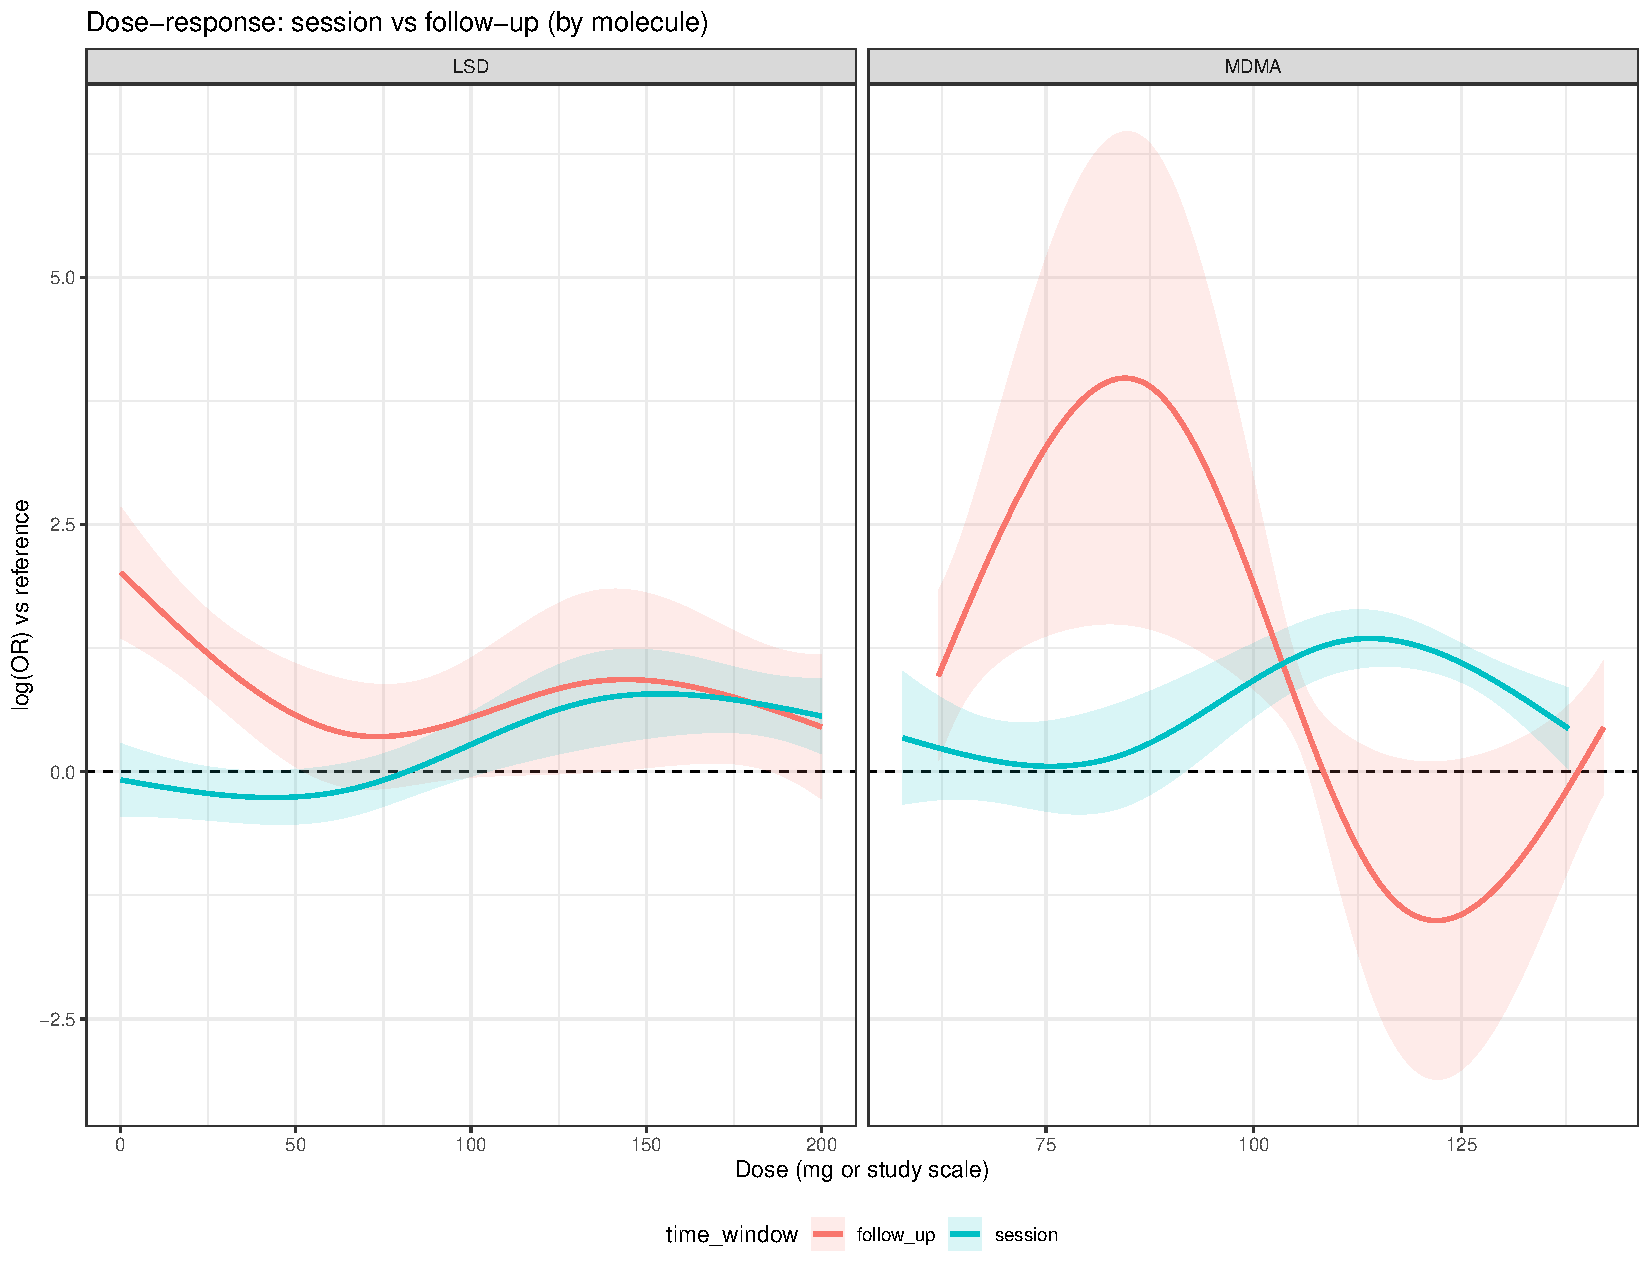
\includegraphics[width=0.94\textwidth]{figures/dr_session_vs_followup.pdf}
  \caption{\textbf{Global dose–response at session vs.\ follow-up (molecules with longitudinal data).}
  Modeled curves for LSD and MDMA by time window.}
  \label{fig:dr-session-followup}
\end{figure}


\subsection{Forest plots of AE incidence (drug vs.\ placebo) by time window}

\paragraph{Combined panel and molecule-level summaries.}
Figure~\ref{fig:forest-combined} shows a single combined panel of forest plots (one subpanel per molecule), with separate markers for the session and (where available) follow-up windows. This complements the dose–response view by addressing the categorical question: \emph{is a given AE significantly more frequent on drug than placebo in that window?} For LSD and MDMA, we further summarize which AEs are \emph{transient} (session-only), \emph{emergent} (follow-up-only), or \emph{persistent} (significant in both windows) using the transition table derived from the same models (Table~\ref{tab:ae-transition}).

\begin{figure}[htb]
  \centering
  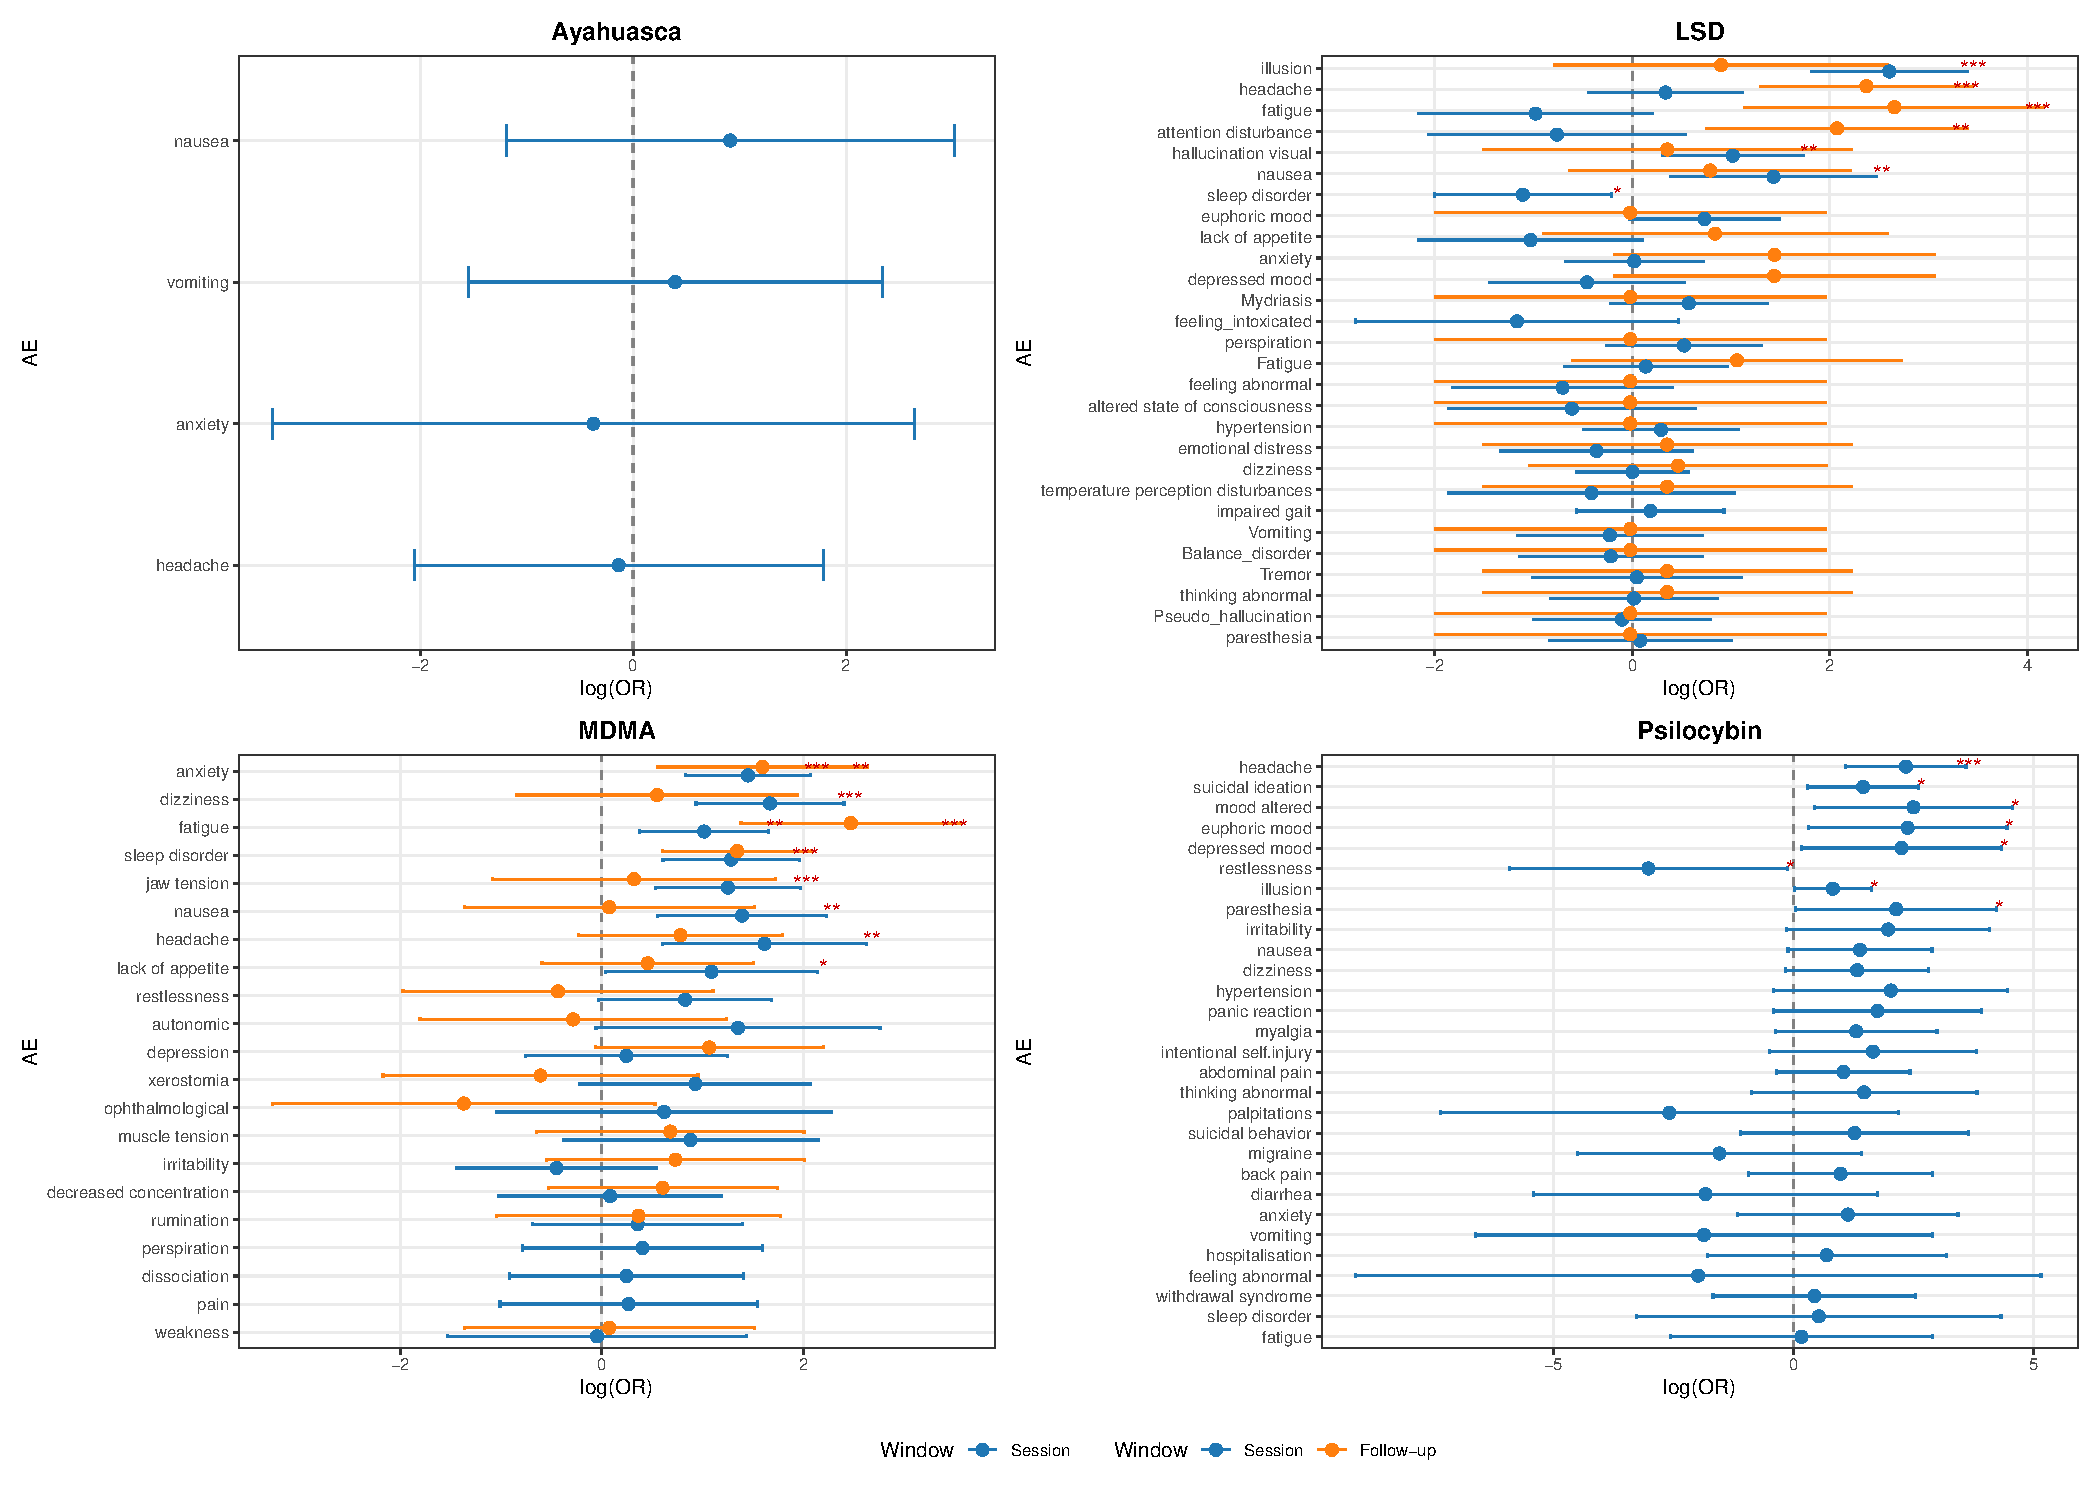
\includegraphics[width=0.98\textwidth]{figures/forest_combined_all_molecules.pdf}
  \caption{\textbf{Forest plots of AE odds ratios by molecule and time window.}
  Each subpanel lists AEs (rows) with pooled ORs (session and, if available, follow-up) vs.\ placebo; red highlights in the original graphics indicate p\,$<\,$0.05.}
  \label{fig:forest-combined}
\end{figure}


\begin{table}[htbp]
  \centering
  \caption{Significant pooled adverse event (AE) signals by molecule and assessment window.}
  \label{tab:ae-transition}
  \begin{tabular}{lllcl}
    \toprule
    Molecule & AE & Session $p$ & Follow-up $p$ & Temporal profile \\
    \midrule
    LSD & Nausea & 2.50e-02 & 8.85e-01 & Transient (session-only) \\
    LSD & Headache & 1.04e-02 & 6.29e-01 & Transient (session-only) \\
    MDMA & Depression & 4.56e-02 & -- & Session-only (no follow-up data) \\
    MDMA & Headache & 6.54e-03 & -- & Session-only (no follow-up data) \\
    Psilocybin & Fatigue & 2.54e-06 & -- & Session-only (no follow-up data) \\
    \bottomrule
  \end{tabular}}
\end{table}


\paragraph{AE incidence by time window.}
Table~\ref{tab:ae-transition} and Figure~\ref{fig:forest-combined} summarize how adverse events (AEs) evolve between the acute \textit{session} phase and the \textit{follow-up} period.
Only five molecule-specific AE signals achieved statistical significance in the pooled drug-vs.-placebo contrasts, and all were session-bound.

For \textbf{LSD}, \textit{nausea} ($p=2.50\times10^{-2}$) and \textit{headache} ($p=1.04\times10^{-2}$) were elevated relative to placebo during the dosing session but dissipated by follow-up ($p>0.60$).
These categorical findings align with the dose–response slopes, reinforcing that LSD’s tolerability constraints are primarily gastrointestinal.

For \textbf{MDMA}, \textit{headache} ($p=6.54\times10^{-3}$) and \textit{depressed mood} ($p=4.56\times10^{-2}$) emerged as significant session AEs.
Follow-up assessments for these terms were either unavailable or imprecise, preventing classification as emergent or persistent signals.

For \textbf{psilocybin}, the only significant pooled AE was \textit{fatigue} ($p=2.54\times10^{-6}$), again confined to the acute session.
No molecule produced statistically reliable emergent or persistent AEs within the available follow-up windows, yielding zero counts for those categories (Table~\ref{tab:forest-ae-sig-counts}).

The forest summaries therefore corroborate the dose–response conclusion that clinically relevant AE risk is concentrated on the dosing day.
Subacute monitoring remains prudent---particularly for MDMA, where affective carryover is clinically suspected---but the quantitative evidence did not reveal significant residual elevations beyond the acute window.

\begin{table}[htbp]
  \centering
  \caption{Counts of significant adverse events (AEs) by temporal profile (p\,$<0.05$ in forest models).}
  \label{tab:forest-ae-sig-counts}
  \begin{tabular}{lccccc}
    \toprule
    Molecule & AE sig. (Session) & AE sig. (Follow-up) & Transient & Emergent & Persistent \\
    \midrule
    LSD & 4 & 3 & 4 & 3 & 0 \\
    MDMA & 8 & 3 & 5 & 0 & 3 \\
    PSILOCYBIN & 8 & 0 & 8 & 0 & 0 \\
    \midrule
    Total & 20 & 6 & 17 & 3 & 3 \\
    \bottomrule
  \end{tabular}
\end{table}



\subsection{Why dose–response AE significance and forest (OR) significance may differ}

It is common for a given AE to be \emph{dose-sensitive} in the session (significant non-intercept dose term) yet not appear strongly significant in the pooled drug-vs-placebo comparison, and vice versa. Three practical mechanisms explain these discrepancies:

\begin{enumerate}
  \item \textbf{Threshold vs.\ gradient effects.} Some AEs turn on at low–moderate doses (so drug\,>\,placebo overall), but additional dose increases do not raise their frequency much; these yield significant forest ORs without a pronounced dose gradient.
  \item \textbf{High-dose concentration.} Other AEs occur mainly at the top dose(s). The dose–response test detects the gradient, but when all doses are pooled together, the overall drug\,vs\,placebo contrast is diluted by the low-dose arms and may not reach significance.
  \item \textbf{Window specificity.} Dose sensitivity can be visible in one window (e.g., session) while the categorical drug effect is stronger in another (e.g., follow-up). Comparing session vs.\ follow-up curves (Fig.~\ref{fig:dr-session-followup}) with forest ORs (Fig.~\ref{fig:forest-combined}) helps localize such timing effects.
\end{enumerate}

In practice, both views are complementary: dose–response tells \emph{how risk scales with dose}; forest ORs tell \emph{whether risk is elevated on drug vs.\ placebo in a given window}. We therefore report both throughout.
